\chapter{Introducción}
\label{cap:introduccion}

\chapterquote{La inteligencia es la habilidad de adaptarse a los cambios}{Stephen Hawking}

\begin{resumen} En este capítulo se explicará la motivación de este trabajo (Sección \ref{cap1:sec:Motivacion}), los objetivos que se quieren lograr (Sección \ref{cap1:sec:Objetivos}) y la estructura de esta memoria (Sección \ref{cap1:sec:Estructura}). 
\end{resumen}
\section{Motivación}
\label{cap1:sec:Motivacion}

Los seres humanos siempre hemos tenido la necesidad inherente de comunicarnos, y quien no es capaz de hacerlo generalmente acaba excluido. Y esa es la palabra clave, comunicación. Su origen proviene del latín, “\textit{communicare}” difundir, y este de “\textit{communis}” común. Gracias a ello, hemos podido llegar hasta donde estamos actualmente, una era donde todos pueden tener una voz. Por eso es más importante que nunca no olvidarse de los que tienen dificultades. Eliminar la barrera de la comunicación a la que estamos acostumbrados como es el habla o el lenguaje natural, y hacerla comprensible para todos es un reto que se ha ido superando. \textcolor{blue}{[Quiero que darle un par de vueltas a esto]}

Sin embargo, en las últimas décadas ha habido un avance sin precedentes en el estudio e investigación sobre las discapacidades comunicativas. Estos avances vinieron acompañados de herramientas y sistemas para facilitar la comunicación muchos de los cuales siguen vigentes a día de hoy. Uno de los principales perfiles que utilizan estos sistemas son las  personas con Trastorno del Espectro Autista (TEA)

Sin entrar en gran detalle, podemos encontrar que la gente con \textit{TEA} tienen dificultades en la comunicación verbal, pues a menudo la comunicación no es recíproca o no se realiza en el contexto social adecuado. Respecto a la comunicación no verbal, también sufren dificultades al entender el significado de gestos faciales o expresión corporal de otras personas. Todo esto causa a menudo malentendidos, pues generalmente no se comprende correctamente el contexto y se dificulta la comunicación. 

Para facilitar la comunicación de estos colectivos se utilizan otros medios alternativos como los sistemas pictográficos, que permiten comunicarse mediante imágenes. Estos sitemas pictográficos, al estar compuestos por cientos de pictogramas habitualmente, están agrupados en \textbf{tableros pictográficos}. Estos tableros son superficies donde se colocan pictogramas para formar mensajes. Un ejemplo de tablero es el que vemos en la Figura \ref{fig:tablerofisico}. Hasta hace poco, dichos tableros eran creados a mano recortando y pegando los pictogramas pero con el tiempo se han desarrollado herramientas informáticas enfocadas a trabajar con tableros y pictogramas.

% TODO: \usepackage{graphicx} required
\begin{figure}[h!]
	\centering
	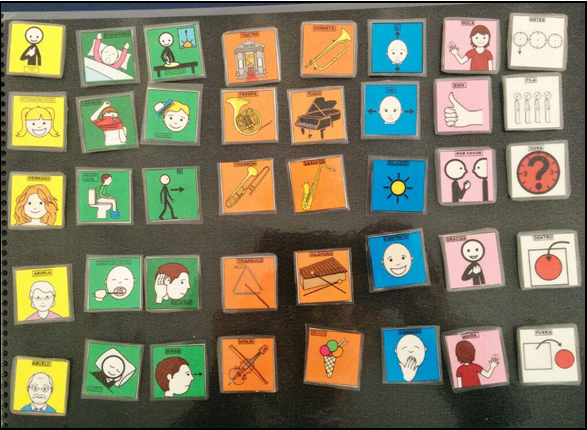
\includegraphics[width=0.7\linewidth]{Imagenes/Bitmap/tablerofisico}
	\caption{Tablero pictográfico en el que el usuario señala lo que quiere comunicar.}
	\label{fig:tablerofisico}
\end{figure}

Todas estas herramientas suelen tener cada una  sus características y funcionalidades únicas. Aun así no existe una alternativa clara que reúna las herramientas necesarias para poder realizar materiales con amplia libertad. A menudo se abusan de tableros de tamaño fijo que limitan la creatividad de quienes crean estos materiales. Por ejemplo, en las aplicaciones mencionadas previamente podemos ver que falta algún tipo de cuadrícula en el tablero para que a la hora de insertar los pictogramas estos queden perfectamente colocados y el tablero tenga una mejor apariencia visual.

En este contexto, la finalidad es crear una herramienta que unifique las mejores características de cada aplicación, además de permitir crear y editar tableros en un mismo lugar con la mayor facilidad y libertad posible. Afortunadamente, ya existe una base sobre la que apoyarse, gracias a proyectos anteriores.







\section{Objetivos}
\label{cap1:sec:Objetivos}

Teniendo en cuenta todos los temas que hemos tratado en la introducción, el objetivo principal de este trabajo es desarrollar una aplicación web multiplataforma que permitirá la creación y edición de tableros interactivos. En la aplicación también se incorporarán herramientas de búsquedas de pictogramas por palabras y traducción de texto a pictograma. 

Respecto a la interacción con los tableros, se hará por medio de componentes configurables, los cuales aportarán algún tipo de interacción con el usuario final, como desplegar un tablero de pictogramas o colocar un pictograma en un hueco.

Para poder cumplir todos los objetivos mencionados se tendrá como referencia los TFG y TFM de Pictar y PicTableros. También se hará una labor de investigación en busca de nuevas tecnologías y herramientas con las que trabajar para desarrollar la aplicación. 

La forma en la que se comprobará el estado de los objetivos y su evolución será por medio de reuniones con los directores del TFG donde se analizará el trabajo realizado para ver el progreso, la forma en la que se implementan los objetivos, y sugerencias para no pausar el progreso.

\textcolor{blue}{¿Podemos poner el inestimable apoyo que nos proporcionáis para animarnos a continuar?}





\section{Estructura de la memoria}
\label{cap1:sec:Estructura}

La estructura para memoria se encuentra dividida en [x] capítulos, a continuación se explicará brevemente su contenido. --según avancemos habrá que ir completándolo--
\begin{itemize}
	\item En los capítulos 1 y 2 se expondrá el contexto bajo el cual se ha realizado el trabajo junto a la motivación y objetivos para realizarlo.
	\item En el capítulo 3 se explicará qué es un pictograma y los distintos sistemas de comunicación basados en ellos. Además se analizarán las distintas herramientas relacionadas con pictogramas haciendo énfasis en la edición de tableros.
\end{itemize}	




